\section{Modello di Ising 1D}

Il modello di Ising 1D è uno dei pochi modelli della meccanica statistica che presenta una soluzione esatta.
Il reticolo che prendiamo in considerazione in questo caso è lineare, tale per cui ogni sito reticolare presenta 
solo due primi vicini. Lavorando con condizioni periodiche al contorno, l'N-esimo spin diventa un vicino del 
primo ed il sistema si chiude ad anello, come è possibile apprezzare in Figura \ref{fig: Ising1D_pbc}.

\begin{figure}[h!]
    \centering
    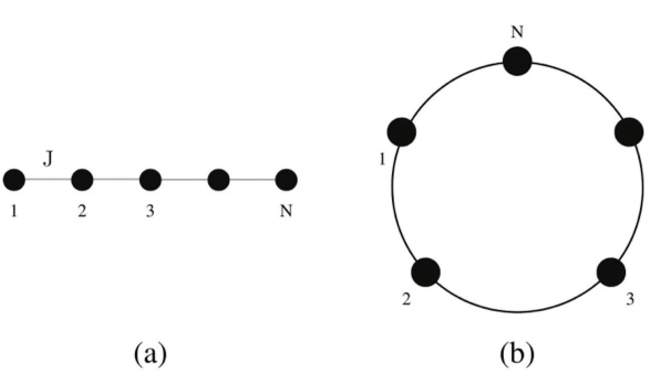
\includegraphics[width=0.7\textwidth]{Immagini/Ising1D_pbc.png}
    \caption{L'immagine (a) è un esempio di modello di Ising 1D senza pbc, mentre in (b) si può apprezzare 
    come la catena si chiuda su se stessa nel caso di condizioni periodiche al contorno. }
    \label{fig: Ising1D_pbc}
\end{figure}

Sebbene il modello di Ising 1D ammetta soluzione esatta, è istruttivo lavorare inizialmente con una teoria di campo 
medio, in cui il termine d'interazione presente nell'Hamiltoniana viene sostituito da un termine efficace (di campo 
medio appunto), andando a trascurare le fluttuazioni degli spin.





\subsection{Teoria di campo medio}

Il punto di partenza di una teoria di campo medio è la semplificazione del temine d'interazione presente nell'Hamiltoniana. Nel  
caso del modello di Ising mono-dimensionale l'interazione fra spin primi vicini può essere riscritta come

\begin{equation}
    \sigma_i \sigma_j\,=\,\left(\sigma_i\,-\,m\,+\,m\right)\left(\sigma_j\,-\,m\,+\,m\right)\,=\,-m^2\,+\,m\sigma_i\,+\,m\sigma_j\,+\,\left(\sigma_i\,-\,m\right)\left(\sigma_j\,-\,m\right),
    \label{eq: int_mf}
\end{equation}

dove l'ultimo termine della somma misura le fluttuazioni fra spin. L'approssimazione di campo medio consiste nel trascurare 
completamente l'ultimo termine, in modo tale che tutti gli spin risultino essere disaccoppiati fra loro e risulti più immediato il 
calcolo della funzione di partizione. L'Hamiltoniana di campo medio risulta quindi 

\begin{equation}
    H_{MF}\,=\,-\frac{J}{2} \sum_{\left<i,j\right>} \left[-m^2\,+\,m\left(\sigma_i\,+\,\sigma_j\right)\right]\,-\,h\sum_{i}\sigma_i,
    \label{eq: ham_mf}
\end{equation}

da cui è immediato il calcolo della funzione di partizione 

\begin{equation}
    Q_{MF}\,=\,\sum_{\left\{\sigma\right\}} e^{-\beta H_{MF}}\,=\,\exp{\left(-\frac{\beta J m^2 N n_{nn}}{2}\right)} \left\{2 \cosh{\left[\beta \left(J n_{nn} m\,+\,h\right)\right]}\right\}^N.
    \label{eq: part_MF_Ising1D}
\end{equation}

Nella relazione precedente la quantità $n_{nn}$ è il numero il numero di coordinazione del reticolo, ossia il numero di primi vicini per la 
geometria presa in considerazione. L'energia libera per particella è data da 

\begin{equation}
    \frac{F}{N}\,=\,-\frac{k_B T}{N} \ln{\left(Q_{MF}\right)}\,=\,\frac{JM^2n_{nn}}{2}\,-\,\frac{1}{\beta}\ln{\left\{2 \cosh{\left[\beta\left(h\,+\,Jn_{nn}m\right)\right]}\right\}}
    \label{eq: freeE_MF_Ising1D}
\end{equation}

da cui è possibile ricavare tutta la termodinamica del sistema.



\subsubsection{Magnetizzazione}

La magnetizzazione si ricava a partire dall'energia libera per spin mediante una derivata rispetto al campo magnetico $h$. 
La relazione che si ottiene è nota come \textit{equazione di Bragg-Williams}, che può essere espressa nella forma 

\begin{equation}
    \tanh^{-1}{\left(m\right)}\,=\,\frac{h\,+\,n_{nn}Jm}{k_B T}
    \label{eq: BW_equation}
\end{equation}

Nel caso in cui il campo magnetico è identicamente nullo, è necessario distinguere due casistiche in base alla temperatura del sistema. 
In primo luogo è necessario introdurre la temperatura critica 

\begin{equation}
    T_c\,=\,\frac{n_{nn}J}{k_B},
    \label{eq: tc_Ising1D_MF}
\end{equation}

che consente di riscrivere il secondo membro dell'equazione di Bragg-Williams in funzione del rapporto fra $T_c$ e la temperatura 
a cui il sistema si trova. Così facendo risulta evidente che quando $T\,>\,T_c$ l'unica soluzione possibile dell'equazione 
\eqref{eq: BW_equation} è $m\,=\,0$, ossia mancanza di magnetizzazione finita. Nel caso opposto, ossia con $T\,<\,T_c$, si hanno 
tre possibili valori di $m$, ossia $0,\,\pm m_0$, con $m_0$ quantità finita. L'energia libera consente di identificare quale 
sia la soluzione fisica, poichè come è possibile osservare in Figura \ref{fig: FE_Ising1D_MF} quando la temperatura scende al 
di sotto di quella critica $F$ passa da un regime in cui è presente un solo minimo in $m\,=\,0$ ad un regime con due minimi 
equivalenti in $m\,=\,\pm m_0\,\neq\,0$. 

\begin{figure}[h!]
    \centering
    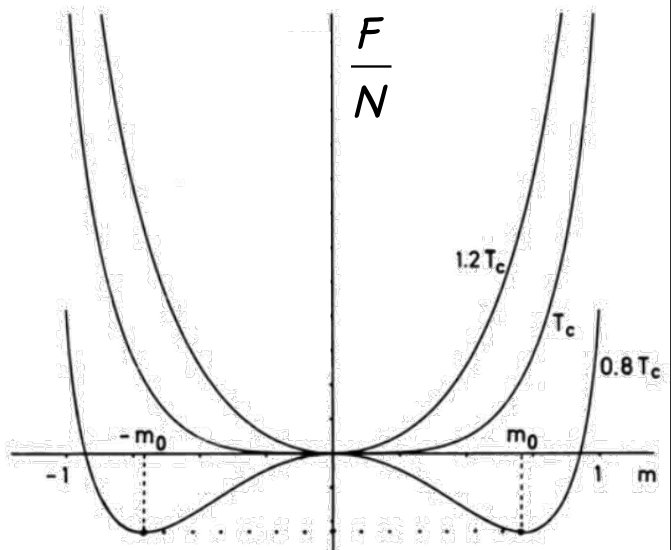
\includegraphics[width=0.7\textwidth]{Immagini/FE_Ising1D_MF.png}
    \caption{ Energia libera per particella al variare della temperatura del sistema. Quando la temperatura è maggiore o uguale 
    di quella critica è presente un solo minimo in $m\,=\,0$, mentre al di sotto sono presenti due minimi globali equivalenti e 
    simmetrici rispetto ad $m\,=\,0$, che è un massimo locale. Immagine da \cite{galliFSA}.}
    \label{fig: FE_Ising1D_MF}
\end{figure}

Questi due valori d'equilibrio della magnetizzazione sono perfettamente simmetrici in assenza di campo magnetico: una 
rottura spontanea della simmetria per inversione di spin è necessaria per far si che il sistema realizzi uno dei due stati di 
minimo globale dell'energia libera. 

Nel caso di campo magnetico esterno diverso da zero non si osserva più la simmetria caratteristica del caso con $h\,=\,0$ e l'
allineamento fra spin concorde con il verso di $h$ risulta essere energeticamente favorito.



\subsubsection{Esponenti critici}

E' possibile caratterizzare il comportamento di un certo sistema nell'intorno del punto critico in termini di leggi di potenza 
che presentano un set di esponenti critici. La seguente analisi è rivolta a 

\begin{table}[h!]
    \centering
    \begin{tabular}{|>{\centering\arraybackslash}p{2cm}|>{\centering\arraybackslash}p{11cm}|}
    \hline
    \textbf{Esponente} & \textbf{Significato fisico} \\ 
    \hline
    $\alpha$ & Descrive l'andamento del calore specifico al punto critico \\ 
    \hline
    $\beta$ & Descrive l'andamento del parametro d'ordine al punto critico \\ 
    \hline
    $\gamma$ & Descrive l'andamento della suscettività al punto critico \\ 
    \hline
    $\delta$ & E' legato all'equazione di stato alla temperatura critica \\ 
    \hline
    \end{tabular}
    \caption{Esponenti critici e relativo significato}
\end{table}

Procediamo ora al calcolo degli esponenti critici $\beta$ e $\delta$ per il modello di Ising mono-dimensionale. L'equazione di Bragg-Williams 
è uno strumento importante per il calcolo di $\beta$, poichè per $T\,\to\,T^-_c$ la magnetizzazione è molto minore di uno ed è possibile 
espandere in serie la tangente iperbolica tralasciando i termini di ordine superiore al terzo 

\begin{equation}
    m\,=\,\tanh{\left(m\frac{T_c}{T}\right)}\,\simeq\,m\frac{T_c}{T}\,-\,\frac{m^3}{3}\left(\frac{T_c}{T}\right)^3
    \label{eq: beta_fp_Ising1D_MF}
\end{equation}

in modo tale che, in seguito ad posto ad uno il fattore moltiplicativo del termine di grado 3, è possibile ricavare la 
magnetizzazione in funzione della differenza fra la temperatura critica e quella a cui si trova il sistema. Dato che 

\begin{equation}
    m\,\simeq\,\sqrt{3\left(\frac{T_c\,-\,T}{T_c}\right)}, 
    \label{eq: beta_sp_Ising1D_MF}
\end{equation}

l'esponente critico $\beta$ sarà pari ad un mezzo. Il calcolo di $\delta$ fa nuovamente uso dell'equazione di Bragg-Williams, che 
a temperature confrontabili con quella critica e per piccoli valori del campo magnetico, può essere espressa come 

\begin{equation}
    m\,=\,\tanh{\left(\frac{h}{k_BT}\,+\,m\frac{T_c}{T}\right)}\,\simeq\,\frac{h}{k_B T}\,+\,m\frac{T_c}{T}\,-\,\frac{1}{3}\left(\frac{h}{k_B T}\,+\,m\frac{T_c}{T}\right)^3
    \label{eq: delta_fp_Ising1D_MF}
\end{equation}

che porta all'equazione di stato approssimata 

\begin{equation}
    \frac{h}{k_B T}\,=\,m\frac{T\,-\,T_c}{T}\,+\,frac{m^3}{3}.
    \label{eq: beta_sp_Ising1D_MF}
\end{equation}

Considerando l'isoterma critica, il primo termine della somma a secondo membro scompare in modo tale che magnetizzazione e 
campo magnetico siano legati come 

\begin{equation}
    m\,\simeq\,\left(\frac{3h}{k_B T_c}\right)^{\frac{1}{3}},
    \label{eq: beta_tp_Ising1D_MF}
\end{equation}

che di conseguenza consente di identificare come $\delta\,=\,3$.





\subsection{Soluzione esatta}

Considerare un sistema con condizioni periodiche al contorno, come (b) in Figura \ref{fig: Ising1D_pbc}, consente 
di scrivere l'Hamiltoniana in forma simmetrica come 

\begin{equation}
    H\,=\,-J\sum_{i} \sigma_i \sigma_{i+1}\,-\,\frac{h}{2}\sum_{i} \left(\sigma_i\,+\,\sigma_{i+1}\right),
    \label{eq: ising_ham_sim}
\end{equation}

dato che $\sigma_{N+1}\,=\,\sigma_1$. La funzione di partizione del sistema è data dalla somma su tutte le possibili 
configurazioni del sistema, che si traduce in 

\begin{equation}
    Q\left(h,\,T\right)\,=\,\sum_{\sigma_1=\pm 1} \cdots \sum_{\sigma_N=\pm 1} \exp{\left\{\beta\left[J\sum_i \sigma_i \sigma_{i+1}\,+\,\frac{h}{2}\sum_i \left(\sigma_i\,+\,\sigma_{i+1}\right)\right]\right\}}
    \label{eq: part_func}
\end{equation}

Definendo una matrice P come

\begin{equation}
    P = \begin{pmatrix}
    e^{\beta\left(J\,+\,h\right)} & e^{-\beta J} \\\\
    e^{-\beta J} & e^{\beta\left(J\,-\,h\right)}
    \end{pmatrix}
    \label{eq: mat_P}
\end{equation}

è possibile riscrivere la funzione di partizione in termini matriciali

\begin{equation}
    Q\left(h,\,T\right)\,=\,\sum_{\sigma_1=\pm 1} \cdots \sum_{\sigma_N=\pm 1} \langle \sigma_1 | P | \sigma_2 \rangle \langle \sigma_2 | P | \sigma_3 \rangle \cdots \langle \sigma_{N-1} | P | \sigma_N \rangle \langle \sigma_N | P | \sigma_1 \rangle 
    \label{eq: part_func_mat}
\end{equation}

Notando che sono presenti $N\,-\,1$ completezze, è possibile procedere ad una semplificazione estrema della relazione 
\eqref{eq: part_func_mat} che consente di apprezzare come la funzione di partizione altro non sia che la traccia della matrice P 
elevata alla N. 

\begin{equation}
    Q\left(h,\,T\right)\,=\,\sum_{\sigma_1=\pm 1} \langle \sigma_1 | P^N | \sigma_1 \rangle \,=\,Tr\left(P^N\right)\,=\,\lambda_1^N\,+\,\lambda_2^N,
    \label{eq: part_func_simp}
\end{equation}

dove $\lambda_1$ e $\lambda_2$ sono gli autovalori della matrice P. La loro determinazione richiede la soluzione di un problema agli 
autovalori, che porta a 

\begin{equation}
    \lambda_{1,2}\,=\,e^{\beta J} \cosh{\left(\beta h\right)}\,\pm\,\sqrt{e^{- 2 \beta J}\,+\,e^{2 \beta J} \sinh^2{\left(\beta h\right)}}.
    \label{eq: autoval_P}
\end{equation}

Una ottima approssimazione, quando il numero di spin preso in considerazione è elevato, consiste nel trascurare il secondo autovalore 
dato che 

\begin{equation}
    \lim_{N \to \infty} \left(\frac{\lambda_2}{\lambda_1}\right)^N\,=\,0.
    \label{eq: approx_Q}
\end{equation}

L'energia libera di Helmholtz, dalla quale è possibile determinare tutta la termodinamica del sistema, risulta quindi

\begin{equation}
    A\left(h,\,T\right)\,=\,-k_B T \ln{\left[Q\left(h,\,T\right)\right]}\,\simeq\,-Nk_BT \ln{\left(\lambda_1\right)}.
    \label{eq: en_lib}
\end{equation}



\subsubsection{Magnetizzazione}

Dall'energia libera di Helmholtz è possibile ricavare la magnetizzazione per spin, che costituisce il parametro d'ordine del 
sistema in analisi ed in quanto tale consente di caratterizzare le transizioni di fase. In particolare, tale quantità si 
ottiene come derivata di $A\left(h,\,T\right)$ rispetto al campo magnetico applicato, in modo tale che

\begin{equation}
    m\,=\,-\left(\frac{\partial A/N}{\partial h}\right)_T\,=\,\frac{\sinh{\left(\beta h\right)}}{\sqrt{e^{-4\beta J}\,+\,\sinh^2\left(\beta h\right)}}
    \label{eq: magn_Ising1D_corr}
\end{equation}

Notiamo che se $h\,\to\,0$ la magnetizzazione tende ad un valore nullo per ogni temperatura finita. Questo fatto evidenzia 
come sia impossibile avere una transizione di fase a temperatura finita T, come invece sembrava evidente nella teoria di campo medio.
Quando si ha $T\,=\,0$ $m$ satura ad uno per ogni valore del campo magnetico, il che implica spin totalmente allineati; questo significa 
che la temperatura critica $T_c$ coincide con lo zero assoluto. E' anche possibile calcolare la suscettività magnetica, la quale diverge 
quanto $T\,\to\,0$, che è il comportamento che ci si aspetterebbe al punto critico. \newline

Il motivo alla base delle errate previsioni della teoria di campo medio è che tale approccio diventa esatto nel limite in cui 
le fluttuazioni del parametro d'ordine sono molto più piccole del valore effettivo dello stesso al punto critico. Il \textit{criterio di Ginzburg} 
afferma che per sistemi tipo Ising, il campo medio fornisce soluzioni esatte solamente per dimensioni del reticolo superiori a 
quattro. Il miglioramento delle previsioni all'aumentare della dimensionalità risulta evidente dal confronto fra gli esponenti 
critici calcolati in campo medio e quelli ottenuti in modo analitico o computazionale mediante simulazioni Monte-Carlo.

\begin{table}[h!]
    \centering
    \begin{tabular}{|>{\centering\arraybackslash}p{3cm}|>{\centering\arraybackslash}p{3cm}|>{\centering\arraybackslash}p{3cm}|>{\centering\arraybackslash}p{3cm}|}  
    \hline
    \textbf{Esponente} & \textbf{Mean-field} & \textbf{Ising 2D} & \textbf{Ising 3D}\\ 
    \hline
    $\alpha$ & 0 & 0 & 0.119 $\pm$ 0.006 \\
    \hline
    $\beta$ & 1/2 & 1/8 & 0.326 $\pm$ 0.004 \\
    \hline
    $\gamma$ & 1 & 7/4 & 1.239 $\pm$ 0.003 \\
    \hline
    $\delta$ & 3 & ? & 4.80 $\pm$ 0.05 \\
    \hline
    $\nu$ & 1/2 & 1 & 0.627 $\pm$ 0.002 \\
    \hline
    \end{tabular}
    \caption{Confronto fra esponenti critici calcolati in campo-medio e in modo analitico/numerico per modelli di Ising 2D e 3D.}
\end{table}



\subsubsection{Correlazioni fra spin}

Consideriamo ora un modello di Ising costituito da un reticolo lineare aperto, senza più condizioni al contorno periodiche, 
come quello in Figura \ref{fig: Ising1D_open}. 

\begin{figure}[H]
    \centering
    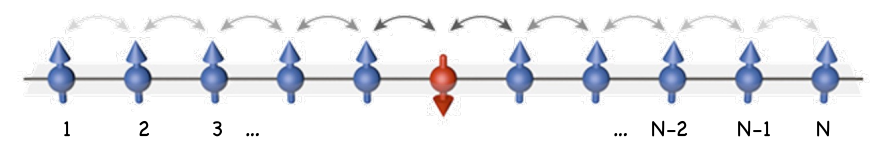
\includegraphics[width=0.7\textwidth]{Immagini/Ising1D_open.png}
    \caption{Esempio di catena di spin per la determinazione della funzione di correlazione fra due spin. Immagine da \cite{galliFSA}.}
    \label{fig: Ising1D_open}
\end{figure}

La funzione di correlazione fra due spin $\sigma_i$ e $\sigma_j$ è definita come

\begin{equation}
    G_{ij}\,=\,\left<\sigma_i \sigma_j\right>\,-\,\left<\sigma_i\right>\left<\sigma_j\right>
    \label{eq: def_corr_fun_Ising1D}
\end{equation}

e consente di valutare se due spin sono correlati o meno. Nel caso del modello di Ising 1D la funzione di correlazione 
risulta essere

\begin{equation}
    G_{i, i+r}\,=\,\left(\tanh{\beta J}\right)^r.
    \label{eq: Ising1D_cor}
\end{equation}

Dall'equazione \eqref{eq: Ising1D_cor} è possibile determinare quale sia la lunghezza di correlazione esprimendo la 
$G_{i, i+r}$ come una funzione esponenzialmente decadente della separazione $r$ fra gli spin in analisi. 

\begin{equation}
    G_{i, i+r}\,=\,e^{r\left[\ln{\left(\tanh{\beta J}\right)}\right]}\,=\,e^{-r/\xi},
    \label{eq: Ising1D_corr_exp}
\end{equation}

da cui risulta che la lunghezza di correlazione è pari a 

\begin{equation}
    \xi\,=\,-\frac{1}{\ln{\left[\tanh{\left(J/k_B T\right)}\right]}}.
    \label{eq: lungh_corr}
\end{equation}

Notiamo che la lunghezza di correlazione è sempre maggiore o uguale a zero. Inoltre, quando la temperatura tende a zero, 
$\xi$ diverge ad infinito. Il fatto che questo accada solamente a temperatura nulla evidenzia come non si abbia correlazione 
(e di conseguenza ordine) a lungo raggio fra gli spin per ogni $T\,\neq\,0$.



\subsubsection{Domain walls}

I domain walls sono i bordi che delimitano due domini magnetici caratterizzati da orientamenti differenti dei momenti magnetici. 
Studiare quale sia l'effetto di queste interfacce sull'energia libera consente di comprende perchè nel modello di Ising 1D vinca il 
disordine (in assenza di campo magnetico) ad ogni temperatura finita. Consideriamo un sistema aperto (quindi senza pbc) a $T\,=\,0$ 
e campo magnetico nullo. Esso si trova nel suo ground state, ossia tutti gli spin presentano lo stesso orientamento. La più semplice 
eccitazione di un sistema di questo genere consiste nella formazione di una singola interfaccia, come riportato in Figura 
\ref{fig: dw_Ising1D}, che separi totalmente spin up e spin down.

\begin{figure}[H]
    \centering
    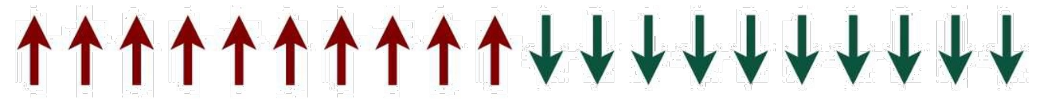
\includegraphics[width=0.7\textwidth]{Immagini/dw_Ising1D.png}
    \caption{Esempio di eccitazione elementare per un modello di Ising 1D. Immagine da \cite{galliFSA}.}
    \label{fig: dw_Ising1D}
\end{figure}

La differenza in energia fra i due stati sopracitati è pari a $2 J$, quindi nel caso di un sistema che presenti una concentrazione 
$x\,=\,M/N$ di domain walls la variazione di energia libera sarà pari a 

\begin{equation}
    \Delta A\,=\,\Delta E\,-\,TS\,=\,2JM\,-\,k_bT\ln{\left(\frac{N!}{M!\left(N\,-\,M\right)!}\right)}
    \label{eq: freeE_dw1_Ising1D}
\end{equation}

Utilizzando la formula di Stirling per espandere i fattoriali, è possibile ottenere la seguente relazione in funzione della concentrazione 
$x$ introdotta in precedenza

\begin{equation}
    \Delta A\,\simeq\,N\left\{2Jx\,+\,k_B T \left[x\ln{\left(x\right)}\,+\,\left(1\,-\,x\right)\ln{\left(1\,-\,x\right)}\right]\right\}
    \label{eq: freeE_dw1_Ising1D}
\end{equation}

Per determinare quale sia la concentrazione all'equilibrio termodinamico si deve minimizzare l'energia libera, ossia la derivata prima 
della stessa rispetto ad $x$ deve essere posta pari a zero. Questo porta a 

\begin{equation}
    x\,=\,\frac{1}{1\,+\,\exp{\left(2 \beta J\right)}}, 
    \label{eq: con_dw_Ising1D}
\end{equation}

ossia una quantità finita per ogni $T \neq 0$. Questo evidenzia come non sia possibile long range order dell'orientazione degli spin e 
di conseguenza la magnetizzazione è identicamente nulla. In 1D, il contributo entropico all'energia libera domina quello energetico, 
favorendo stati di disordine con spin orientati casualmente.